%================================================================
\section{Appendix}\label{sec:Appendix A}
%================================================================

%----------------------------------------------------------------
\subsection{Additional Results}\label{app:additional_results}
%---------------------------------------------------------------- 

%----------------------------------------------------------------
\textbf{Optimzer examination on a spherical harmonic oscillator system without interactions between the bosons.}
%----------------------------------------------------------------

\autoref{fig:alpha_epoch_rwm} displays the evolution of the variational parameter, $\alpha$, from ten different initial starting values in the range $\alpha\in[0.1, 1.0]$ using the RWM sampling algorithm. For most initial $\alpha$-values the ADAM optimizer converges to the optimal variational parameter for the spherical harmonic oscillator, $\alpha^{\mathrm{opt}}=0.5$, although we see that the convergence is a little too slow for the smallest initial $\alpha$ when the learning rate is $0.01$, and the learning rate should maybe be adjusted to $\eta = 0.05$ for faster convergence. When $\eta=0.5$ we see that the initial values close to $\alpha=0.1$ have a hard time converging within the epoch interval. Eventually maybe these also converge to the right value, as the gradients seem to have an easier time finding the optimal variational parameter from $\alpha>\alpha^{\mathrm{opt}}$, however it seems the gradient at an $\alpha$-value far enough away from the optimal seems to have a weak gradient. \autoref{fig:alpha_epoch_lmh} displays the same examinations, only using the LMH sampling algorithm instead. The two plots display very similar results. The only remark to add is that more initial $\alpha$-values seem to have a hard time converging when $\eta=0.5$. 

\begin{figure}[!htb]
\centering
\subfloat[]{{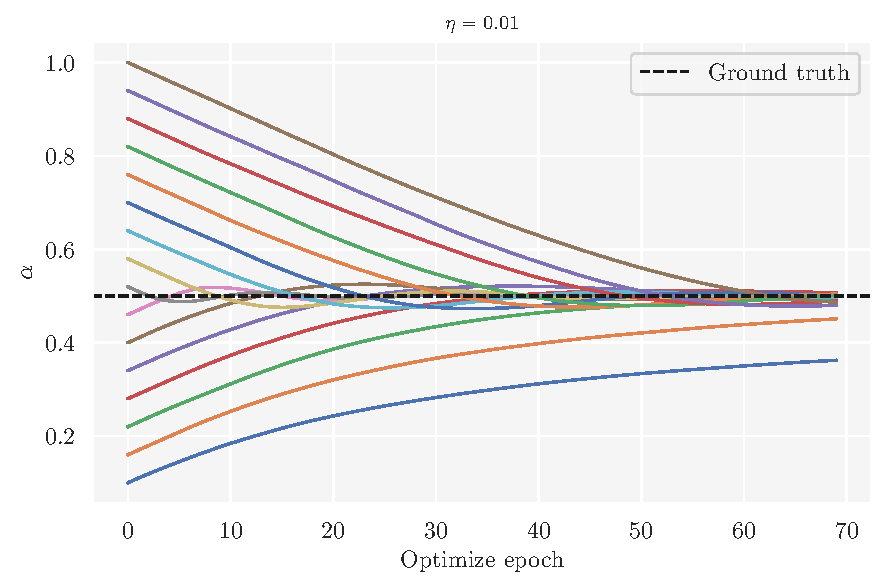
\includegraphics[scale=0.5]{latex/figures/alpha_epoch_rwm_ashonib_eta001.pdf}}}
\qquad
\subfloat[]{{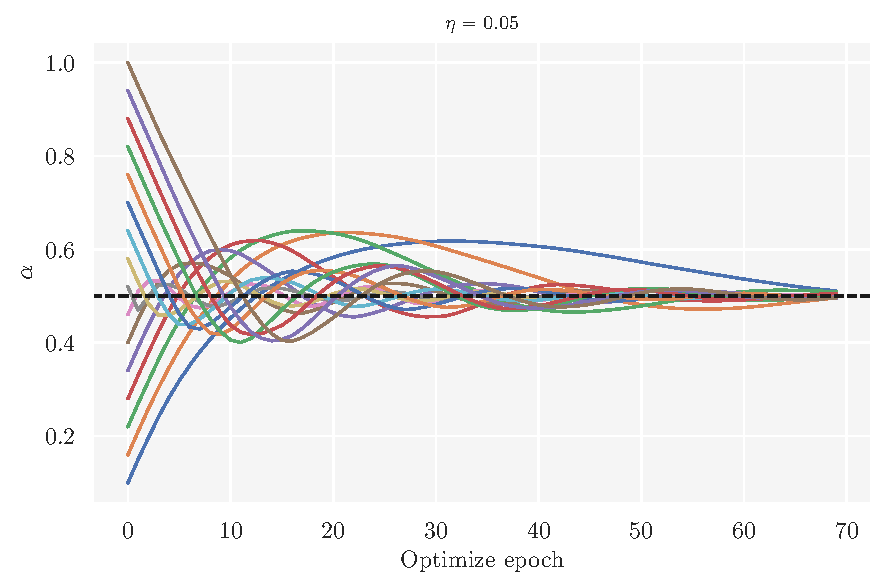
\includegraphics[scale=0.5]{latex/figures/alpha_epoch_rwm_ashonib_eta005.pdf}}}
\qquad
\subfloat[]{{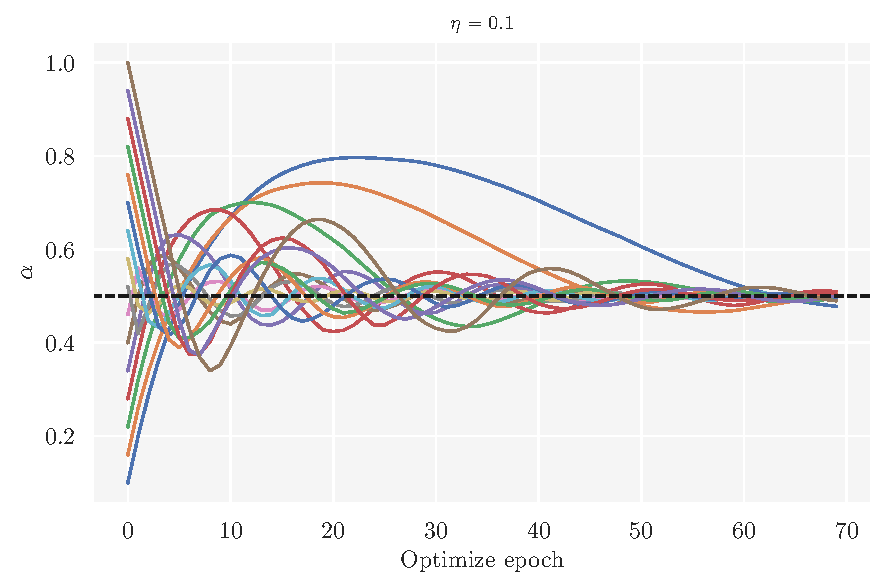
\includegraphics[scale=0.5]{latex/figures/alpha_epoch_rwm_ashonib_eta01.pdf}}}
\qquad
\subfloat[]{{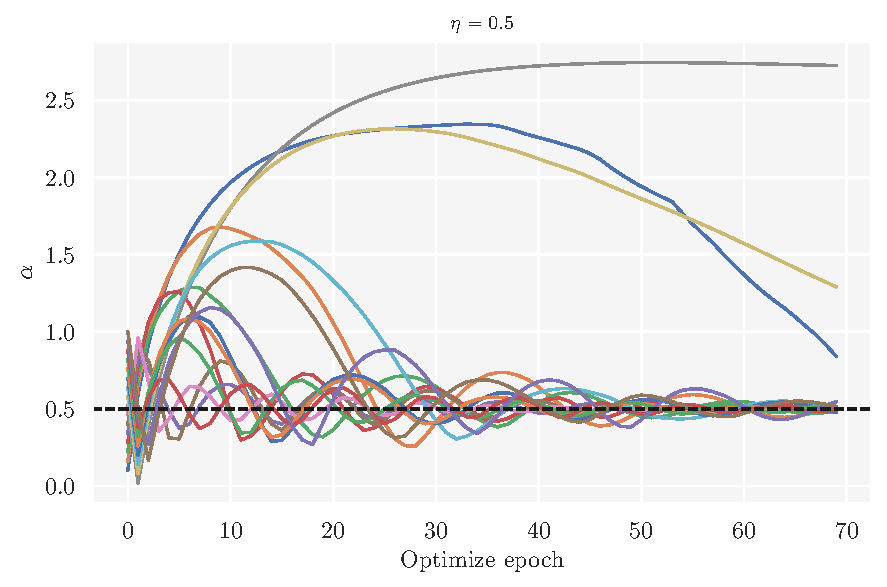
\includegraphics[scale=0.5]{latex/figures/alpha_epoch_rwm_ashonib_eta05.pdf}}}
\caption{Optimization runs with multiple learning rates, $\eta$, examining the convergence of the variational parameter, $\alpha$, starting from initial $alpha\in[0.1,1.0]$ with ten equidistant values, as a function of optimization epochs. The sampling algorithm is the RWM.}
\label{fig:alpha_epoch_rwm}
\end{figure}

\autoref{fig:alpha_epoch_lmh} is similar to \autoref{fig:alpha_epoch_rwm}, only here we use the LMH algorithm. Comparing \autoref{fig:alpha_epoch_rwm} and \autoref{fig:alpha_epoch_lmh} we see no faster convergence for the LMH sampling algorithm than for the RWM sampling algorithm, we see on the contrary that the convergence seem to be a bit faster for the RWM sampling algorithm.

\begin{figure}[!htb]
\centering
\subfloat[]{{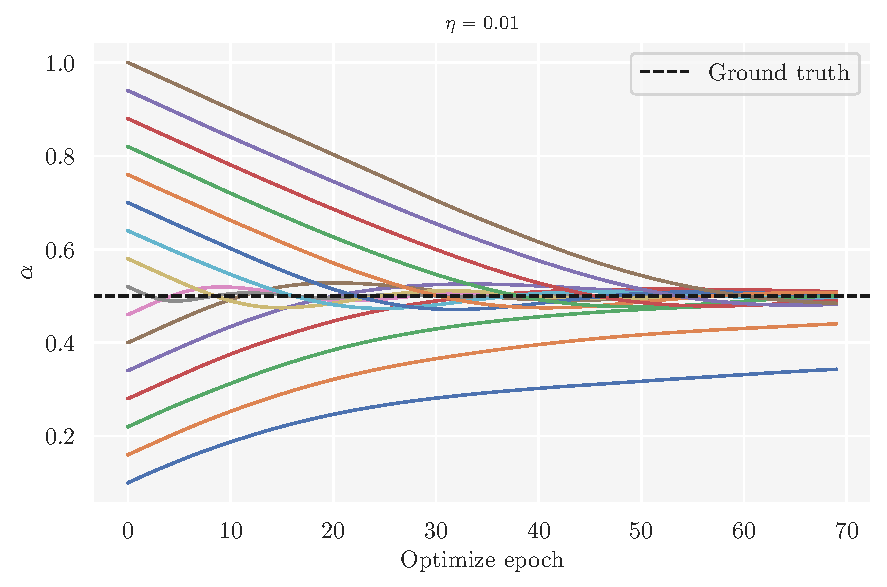
\includegraphics[scale=0.5]{latex/figures/alpha_epoch_lmh_ashonib_eta001.pdf}}}
\qquad
\subfloat[]{{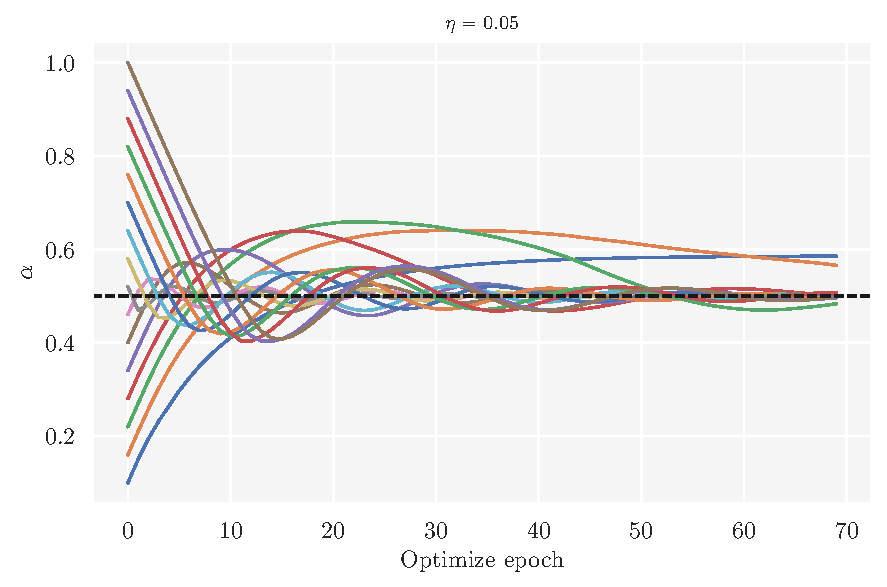
\includegraphics[scale=0.5]{latex/figures/alpha_epoch_lmh_ashonib_eta005.pdf}}}
\qquad
\subfloat[]{{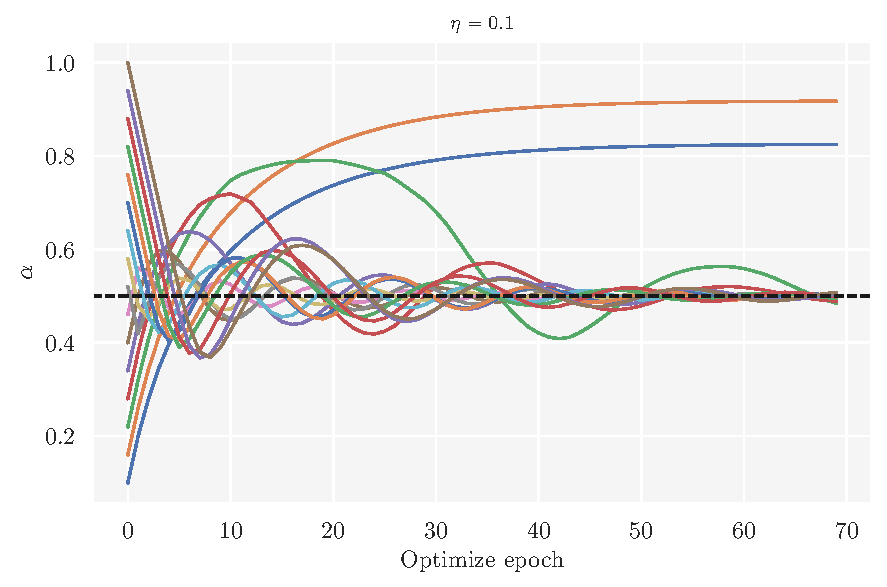
\includegraphics[scale=0.5]{latex/figures/alpha_epoch_lmh_ashonib_eta01.pdf}}}
\qquad
\subfloat[]{{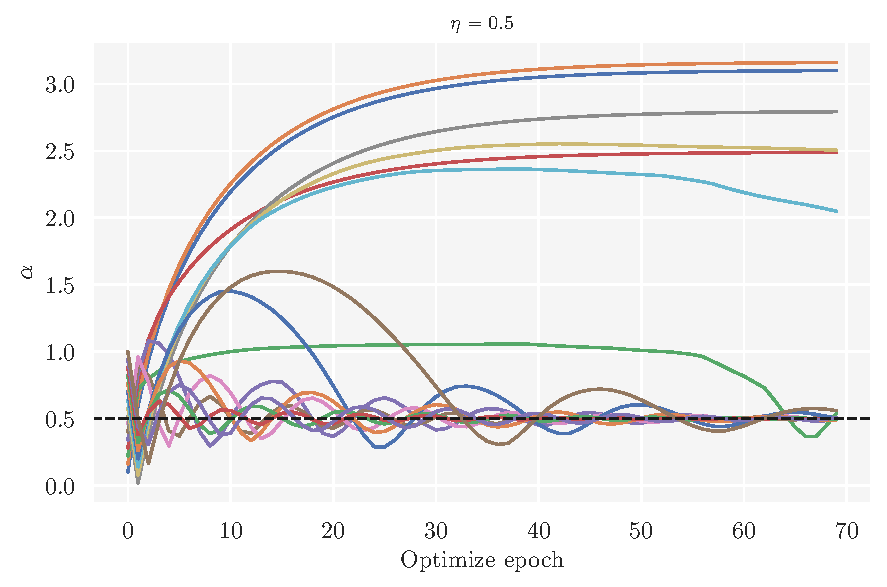
\includegraphics[scale=0.5]{latex/figures/alpha_epoch_lmh_ashonib_eta05.pdf}}}
\caption{Optimization runs with multiple learning rates, $\eta$, examining the convergence of the variational parameter, $\alpha$, starting from initial $\alpha\in[0.1, 1.0]$ with ten equidistant values, as a function of optimization epochs. The sampling algorithm is the LMH.}
\label{fig:alpha_epoch_lmh}
\end{figure}


%----------------------------------------------------------------
\textbf{Energy comparisons for interacting particles in a spherical harmonic oscillator}
%----------------------------------------------------------------
In \autoref{fig:interactions_plot} variational grid searches for the non-interacting case, and $10, 50, 100$ particles with interactions are shown. The $y$-axis displays the energy per particle. A $95$\% confidence interval is shaded in light blue. The minimal energy per particle values together with their standard error, $\sigma$, are tabulated in \autoref{tab:min_energies}. 
\begin{figure}[!htb]
\centering
\subfloat[]{{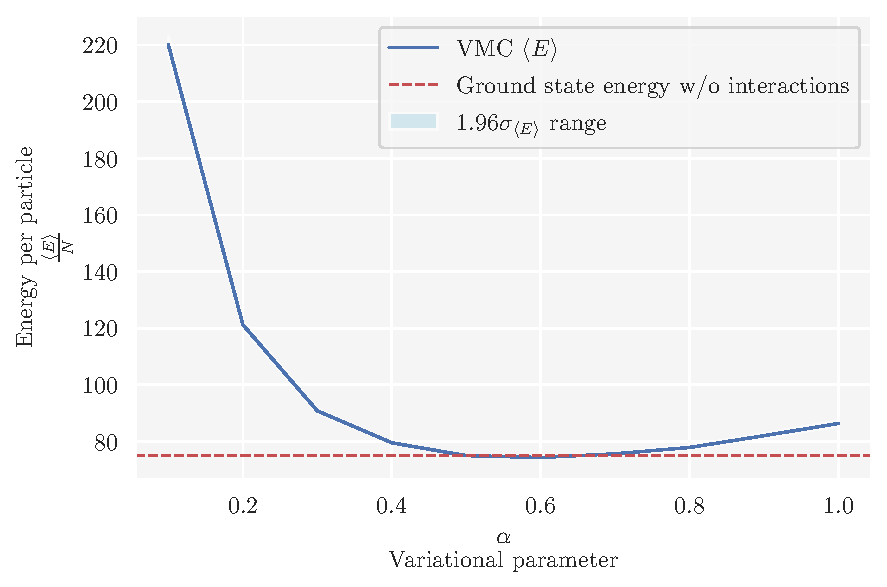
\includegraphics[scale=0.5]{latex/figures/grid_search_analytical_wo_interactions_N_50.pdf}}}
\qquad
\subfloat[]{{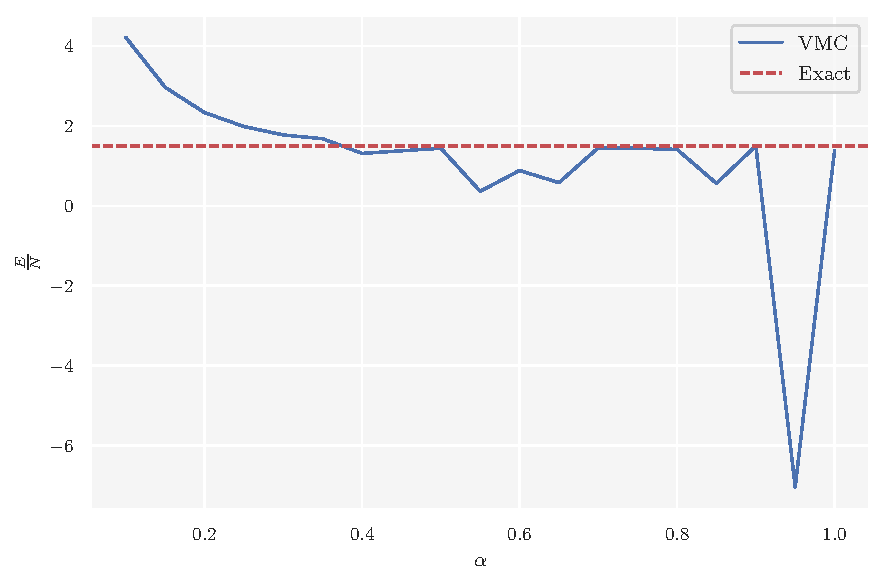
\includegraphics[scale=0.5]{latex/figures/grid_search_analytical_w_interactions_N_10.pdf}}}
\qquad
\subfloat[]{{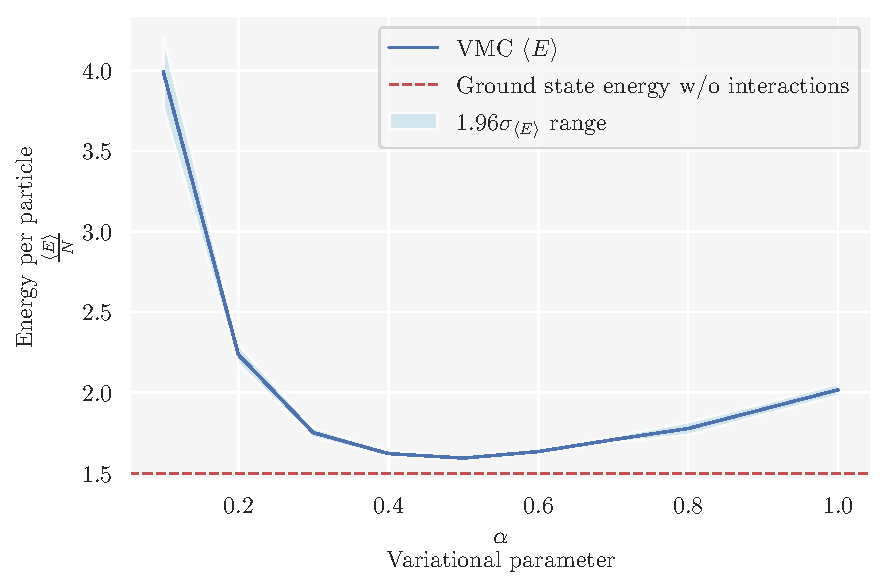
\includegraphics[scale=0.5]{latex/figures/grid_search_analytical_w_interactions_N_50.pdf}}}
\qquad
\subfloat[]{{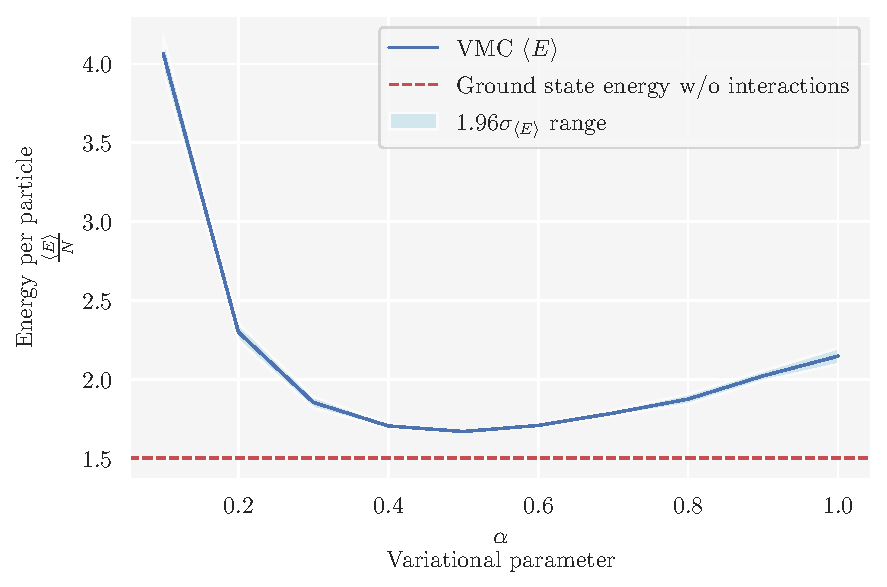
\includegraphics[scale=0.5]{latex/figures/grid_search_analytical_w_interactions_N_100.pdf}}}
\caption{\textbf{(a)} Random Walk Metropolis with 50 non-interacting particles. \textbf{(b)} Random Walk Metropolis with ten interacting particles. \textbf{(c)} Random Walk Metropolis with 50 interacting particles. \textbf{(d)} Random Walk Metropolis with 100 interacting particles.}
\label{fig:interactions_plot}
\end{figure}

\begin{table}[H]
    \centering
    \begin{tabular}{ccccc}
    \hline \hline
        Number of particles & Interactions & $\frac{\expval{E}_{\mathrm{min}}}{N}$ & $\sigma$ & $\alpha^{\mathrm{opt}}$\\
    \hline \hline
        $50$ & Off & $1.500$ & $0\cdot10^{0}$ & $0.5$\\
        $10$ & On & $1.51731$& $8\cdot10^{-5}$& $0.5$ \\
        $50$ & On & $1.59490$& $3\cdot10^{-4}$ &$0.5$ \\
        $100$ & On & $1.66912$ & $3\cdot10^{-4}$ & $0.5$ \\
    \hline \hline
    \end{tabular}
    \caption{The minimal energies of the grid searches for $10, 50, 100$ particles, together with the standard error and the optimal $\alpha$ values. The interactions column displays whether or not the particles are interacting with one another.}
    \label{tab:min_energies}
\end{table}

As you can see in \autoref{tab:min_energies}, the minimal energy per particle is increasing with the number of particles when they are interacting. The density of particles within the potential increases with the number of particles unleashed in the same potential. This leads to more interactions between the particles, and thus a higher energy. Another important quantity, the standard error, is represented with the $95$\% confidence interval $[\mu\pm1.96\sigma]$ by the shaded light blue in \autoref{fig:interactions_plot}. The standard error is relatively small, but it should be possible to see the convex nature of it. It is decreasing from $\alpha=0.1\to\alpha=0.5$, where it increases again. 


\autoref{fig:comparisons_interactions_plot} displays the VMC calculations of the grid searches in \autoref{fig:interactions_plot} all together in one plot. This way it is easier to see the increase in energy per particle as a function of the number of interacting particles. 

\begin{figure}[H]
\begin{center}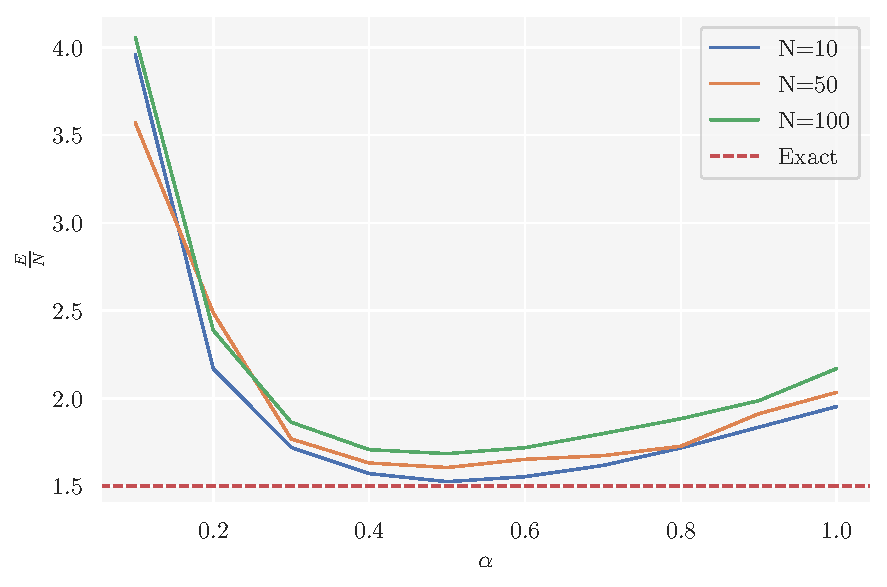
\includegraphics[scale=1.0]{latex/figures/grid_search_analytical_w_interactions_all_N.pdf}
\end{center}
\caption{Random Walk Metropolis energy per particle comparison between $N=10, 50, 100$ interacting particles, and $N=50$ non-interacting particles.}
\label{fig:comparisons_interactions_plot}
\end{figure}

\FloatBarrier

%----------------------------------------------------------------
\subsection{Additional Derivations}\label{app:additional_derivations}
%---------------------------------------------------------------

%----------------------------------------------------------------
\subsubsection*{Error in standard Monte Carlo approximation}
%---------------------------------------------------------------- 
The mean square error $\epsilon_M$ of the Monte Carlo approximation can be written as 
\begin{equation}
    \mathcal{E}_M(\mathbb{E}[f(X)],E_M[f]) = \sqrt{\mathbb{E}[(\mathbb{E}[f(X)]-E_M[f])^2]}. 
\end{equation}
First we recognize the fact that the expecation value of the Monte Carlo approximation is equal to the true expectation value,  $\mathbb{E}[f(X_m)]=\mathbb{E}[f(X)]\quad \forall m\in[1, M]\in\mathbb{N}$, which must be true as $X$ and $X_m$ are identically distributed. We denote the true expecation value, $\mathbb{E}[f(X)]=\mu$. 
We square $\mathcal{E}_M$ 
\begin{equation*}
    \begin{split}
        \mathcal{E}_M^2 &= \mathbb{E}[(\mathbb{E}[f(X)]-E_M[f])^2] \\
        &= \mathbb{E}[\mathbb{E}[f(X)]-2\mathbb{E}[f(X)]E_M[f]+E_M[f]^2] \\
        &= \mathbb{E}[f(X)]-2\mathbb{E}[f(X)]\mathbb{E}[E_M[f]]+\mathbb{E}[E_M[f]^2] \\
        &= \mu^2-2\mu\frac{1}{M}\sum_{m=1}^M\mathbb{E}[f(X_m)] + \frac{1}{M^2}\sum_{m=1}^M\sum_{n=1}^M\mathbb{E}[f(X_m)f(X_n)]. \\
    \end{split}
\end{equation*}
We acknowledge the fact that $f(X_m)$ and $f(X_n)$ are indepent variables, and thus
\begin{equation*}
    \begin{split}
        \mathcal{E}_M^2 &= \mu^2-2\mu\frac{1}{M}\sum_{m=1}^M\mathbb{E}[f(X_m)] + \frac{1}{M^2}\sum_{m=1}^M\sum_{n=1}^N\mathbb{E}[f(X_m)]\mathbb{E}[f(X_n)] \\
        &= \mu^2-2\mu\frac{M\mu}{M} + \frac{1}{M^2}\sum_{m=1}^M(\sum_{m\neq n}\mu^2 + \mathbb{E}[f(X)^2]) \\
        &= -\mu^2+\frac{1}{M^2}((M^2-M)\mu^2 + M\mathbb{E}[f(X)^2]) \\
        &= -\frac{\mu^2}{M} + \frac{1}{M}\mathbb{E}[f(X)^2] \\
        &= \frac{\mathbb{E}[f(X)^2]-\mathbb{E}[f(X)]^2}{M} = \frac{\text{Var}[f(X)]}{M} \\
    \end{split}
\end{equation*}
which leads to 
\begin{equation*}
    \mathcal{E}_M = \frac{\sqrt{\text{Var}[f(X)]}}{\sqrt{M}}.
\end{equation*}



%------------------------------------------------------------------
\subsubsection*{Derivation of the gradient of the local energy with respect to the variational parameters.}
%------------------------------------------------------------------

The expected value of the energy is 
\begin{equation}
    \expval{E} = \int\mathrm{d}\bm{r}E_L(\bm{r};\bm{\alpha})p(\bm{r};\bm{\alpha}),
\end{equation}
which can be rewritten as 
\begin{equation}
    \expval{E} = \frac{\int\mathrm{d}\bm{r}\Psi^*H\Psi}{\int\mathrm{d}\bm{r}\Psi^*\Psi}.
\end{equation}
Now we want to take the derivative of this expression with respect to the variational parameters $\bm{\alpha}$. 
\begin{align*}
    \grad_{\bm{\alpha}}\expval{E} &= \frac{\int\mathrm{d}\bm{r}\qty(\grad_{\bm{\alpha}}\Psi^*H\Psi + \Psi^*H\grad_{\bm{\alpha}})}{\int\mathrm{d}\bm{r}\Psi^*\Psi} - \frac{\qty(\int\mathrm{d}\bm{r}\Psi^*H\Psi)\qty(\int\mathrm{d}\bm{r}\qty[\Psi\grad_{\bm{\alpha}}\Psi^* + \Psi^*\grad_{\bm{\alpha}}\Psi])}{\qty(\int\mathrm{d}\bm{r}\Psi^*\Psi)^2} \\
    &(*)= \frac{\int\mathrm{d}\bm{r}\qty(\grad_{\bm{\alpha}}\Psi^*H\Psi + \Psi\qty[H\grad_{\bm{\alpha}}\Psi]^*)}{\int\mathrm{d}\bm{r}\Psi^*\Psi} - 2\expval{E}\expval{\frac{\grad_{\bm{\alpha}}\Psi}{\Psi}} \\
    &= 2\expval{E\frac{\grad_{\bm{\alpha}}\Psi}{\Psi}} - 2\expval{E}\expval{\frac{\grad_{\bm{\alpha}}\Psi}{\Psi}},
\end{align*}
where we assume hermiticity in the Hamiltonian in (*). Thus, the gradient with respect to the variational parameters becomes 
\begin{equation}
    \grad_{\bm{\alpha}}\expval{E} = 2\qty(\expval{E\frac{\grad_{\bm{\alpha}}\Psi}{\Psi}}-\expval{E}\expval{\frac{\grad_{\bm{\alpha}}\Psi}{\Psi}}).
\end{equation}